\documentclass{standalone}
\usepackage{tikz}
\usetikzlibrary{patterns, positioning}
\usepackage[sfdefault]{ClearSans} %% option 'sfdefault' activates Clear Sans as the default text font
\usepackage[T1]{fontenc}

\begin{document}
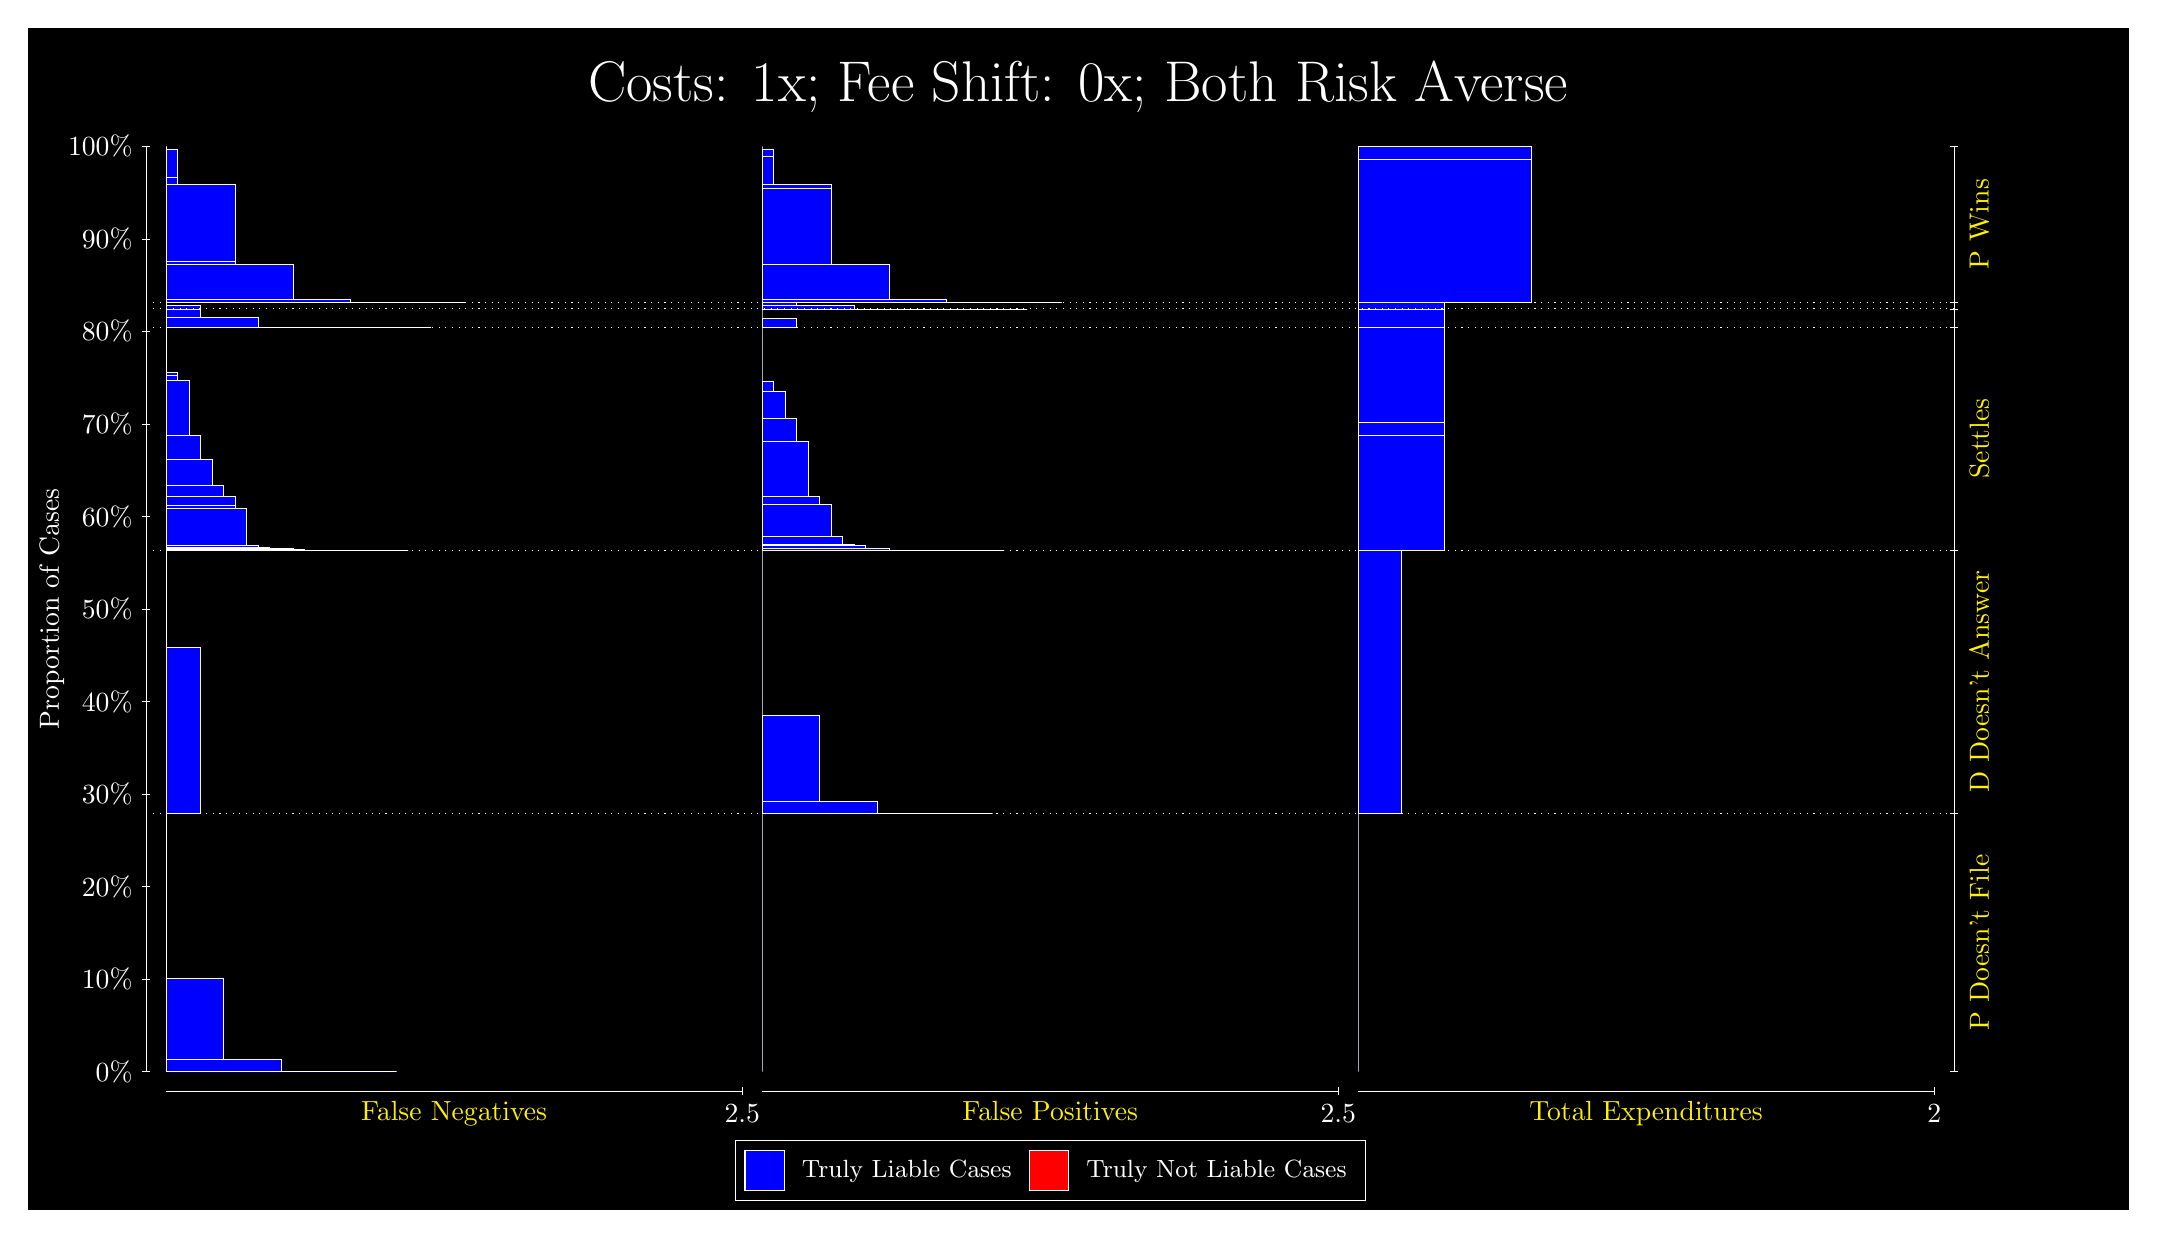
\begin{tikzpicture}
\draw[fill=black] (0,0) rectangle (26.667,15);
\draw[text=white] (0,13.5) rectangle (26.667,15) node[midway] {\huge Costs: 1x; Fee Shift: 0x; Both Risk Averse};
\draw[white, very thin] (1.5,1.75) -- (1.5,13.5);
\node[rotate=90, text=white, anchor=center] at (0.3, 7.625) {Proportion of Cases};
\draw[white, very thin] (1.45,1.75) -- (1.55,1.75);
\node[text=white, anchor=east] at (1.45, 1.75) {0\%};
\draw[white, very thin] (1.45,2.925) -- (1.55,2.925);
\node[text=white, anchor=east] at (1.45, 2.925) {10\%};
\draw[white, very thin] (1.45,4.1) -- (1.55,4.1);
\node[text=white, anchor=east] at (1.45, 4.1) {20\%};
\draw[white, very thin] (1.45,5.275) -- (1.55,5.275);
\node[text=white, anchor=east] at (1.45, 5.275) {30\%};
\draw[white, very thin] (1.45,6.45) -- (1.55,6.45);
\node[text=white, anchor=east] at (1.45, 6.45) {40\%};
\draw[white, very thin] (1.45,7.625) -- (1.55,7.625);
\node[text=white, anchor=east] at (1.45, 7.625) {50\%};
\draw[white, very thin] (1.45,8.8) -- (1.55,8.8);
\node[text=white, anchor=east] at (1.45, 8.8) {60\%};
\draw[white, very thin] (1.45,9.975) -- (1.55,9.975);
\node[text=white, anchor=east] at (1.45, 9.975) {70\%};
\draw[white, very thin] (1.45,11.15) -- (1.55,11.15);
\node[text=white, anchor=east] at (1.45, 11.15) {80\%};
\draw[white, very thin] (1.45,12.325) -- (1.55,12.325);
\node[text=white, anchor=east] at (1.45, 12.325) {90\%};
\draw[white, very thin] (1.45,13.5) -- (1.55,13.5);
\node[text=white, anchor=east] at (1.45, 13.5) {100\%};

\draw[white, very thin] (24.457,1.75) -- (24.457,13.5);
\draw[white, very thin] (24.407,1.75) -- (24.507,1.75);
\node[anchor=west] at (24.407, 1.75) {};
\draw[white, very thin] (24.407,5.0289) -- (24.507,5.0289);
\node[anchor=west] at (24.407, 5.0289) {};
\draw[white, very thin] (24.407,8.3723) -- (24.507,8.3723);
\node[anchor=west] at (24.407, 8.3723) {};
\draw[white, very thin] (24.407,11.204) -- (24.507,11.204);
\node[anchor=west] at (24.407, 11.204) {};
\draw[white, very thin] (24.407,11.436) -- (24.507,11.436);
\node[anchor=west] at (24.407, 11.436) {};
\draw[white, very thin] (24.407,11.519) -- (24.507,11.519);
\node[anchor=west] at (24.407, 11.519) {};
\draw[white, very thin] (24.407,13.5) -- (24.507,13.5);
\node[anchor=west] at (24.407, 13.5) {};

\draw[white, very thin, fill=blue] (1.75,1.75) rectangle (4.6775,1.75);
\draw[white, very thin, fill=blue] (1.75,1.75) rectangle (3.9457,1.7513);
\draw[white, very thin, fill=blue] (1.75,1.7513) rectangle (3.2138,1.9071);
\draw[white, very thin, fill=blue] (1.75,1.9071) rectangle (2.4819,2.9406);
\draw[white, very thin, fill=red] (1.75,2.9406) rectangle (1.75,2.9406);
\draw[white, very thin, fill=blue] (1.75,2.9406) rectangle (1.75,5.0289);
\draw[white, very thin, fill=blue] (1.75,5.0289) rectangle (2.1891,7.133);
\draw[white, very thin, fill=red] (1.75,7.133) rectangle (1.75,7.133);
\draw[white, very thin, fill=blue] (1.75,7.133) rectangle (1.75,8.3723);
\draw[white, very thin, fill=blue] (1.75,8.3723) rectangle (4.8239,8.3723);
\draw[white, very thin, fill=blue] (1.75,8.3723) rectangle (4.2384,8.3723);
\draw[white, very thin, fill=blue] (1.75,8.3723) rectangle (4.092,8.3723);
\draw[white, very thin, fill=blue] (1.75,8.3723) rectangle (3.6529,8.3724);
\draw[white, very thin, fill=blue] (1.75,8.3724) rectangle (3.5065,8.3856);
\draw[white, very thin, fill=blue] (1.75,8.3856) rectangle (3.3602,8.3907);
\draw[white, very thin, fill=blue] (1.75,8.3907) rectangle (3.0674,8.4098);
\draw[white, very thin, fill=blue] (1.75,8.4098) rectangle (2.921,8.4323);
\draw[white, very thin, fill=blue] (1.75,8.4323) rectangle (2.7746,8.8972);
\draw[white, very thin, fill=blue] (1.75,8.8972) rectangle (2.6283,8.9458);
\draw[white, very thin, fill=blue] (1.75,8.9458) rectangle (2.6283,9.0597);
\draw[white, very thin, fill=blue] (1.75,9.0597) rectangle (2.4819,9.1909);
\draw[white, very thin, fill=blue] (1.75,9.1909) rectangle (2.3355,9.5283);
\draw[white, very thin, fill=blue] (1.75,9.5283) rectangle (2.1891,9.8283);
\draw[white, very thin, fill=blue] (1.75,9.8283) rectangle (2.0428,10.526);
\draw[white, very thin, fill=blue] (1.75,10.526) rectangle (1.8964,10.587);
\draw[white, very thin, fill=blue] (1.75,10.587) rectangle (1.8964,10.625);
\draw[white, very thin, fill=red] (1.75,10.625) rectangle (1.75,10.625);
\draw[white, very thin, fill=blue] (1.75,10.625) rectangle (1.75,11.204);
\draw[white, very thin, fill=blue] (1.75,11.204) rectangle (5.1167,11.204);
\draw[white, very thin, fill=blue] (1.75,11.204) rectangle (4.3848,11.204);
\draw[white, very thin, fill=blue] (1.75,11.204) rectangle (3.6529,11.206);
\draw[white, very thin, fill=blue] (1.75,11.206) rectangle (2.921,11.324);
\draw[white, very thin, fill=blue] (1.75,11.324) rectangle (2.1891,11.436);
\draw[white, very thin, fill=red] (1.75,11.436) rectangle (1.75,11.436);
\draw[white, very thin, fill=blue] (1.75,11.436) rectangle (2.1891,11.476);
\draw[white, very thin, fill=red] (1.75,11.476) rectangle (1.75,11.476);
\draw[white, very thin, fill=blue] (1.75,11.476) rectangle (1.75,11.519);
\draw[white, very thin, fill=blue] (1.75,11.519) rectangle (5.5558,11.519);
\draw[white, very thin, fill=blue] (1.75,11.519) rectangle (4.8239,11.519);
\draw[white, very thin, fill=blue] (1.75,11.519) rectangle (4.092,11.554);
\draw[white, very thin, fill=blue] (1.75,11.554) rectangle (3.3602,12.001);
\draw[white, very thin, fill=blue] (1.75,12.001) rectangle (2.6283,12.037);
\draw[white, very thin, fill=blue] (1.75,12.037) rectangle (2.6283,13.012);
\draw[white, very thin, fill=blue] (1.75,13.012) rectangle (1.8964,13.104);
\draw[white, very thin, fill=blue] (1.75,13.104) rectangle (1.8964,13.465);
\draw[white, very thin, fill=red] (1.75,13.465) rectangle (1.75,13.465);
\draw[white, very thin, fill=blue] (1.75,13.465) rectangle (1.75,13.5);
\draw[white, very thin, fill=red] (9.3189,1.75) rectangle (9.3189,1.75);
\draw[white, very thin, fill=blue] (9.3189,1.75) rectangle (9.3189,5.0289);
\draw[white, very thin, fill=red] (9.3189,5.0289) rectangle (12.246,5.0289);
\draw[white, very thin, fill=blue] (9.3189,5.0289) rectangle (12.246,5.0289);
\draw[white, very thin, fill=blue] (9.3189,5.0289) rectangle (11.515,5.0293);
\draw[white, very thin, fill=blue] (9.3189,5.0293) rectangle (10.783,5.1773);
\draw[white, very thin, fill=blue] (9.3189,5.1773) rectangle (10.051,6.2682);
\draw[white, very thin, fill=blue] (9.3189,6.2682) rectangle (9.3189,8.3723);
\draw[white, very thin, fill=red] (9.3189,8.3723) rectangle (12.393,8.3723);
\draw[white, very thin, fill=blue] (9.3189,8.3723) rectangle (12.393,8.3723);
\draw[white, very thin, fill=red] (9.3189,8.3723) rectangle (11.807,8.3723);
\draw[white, very thin, fill=blue] (9.3189,8.3723) rectangle (11.807,8.3723);
\draw[white, very thin, fill=blue] (9.3189,8.3723) rectangle (11.661,8.3724);
\draw[white, very thin, fill=red] (9.3189,8.3724) rectangle (11.515,8.3724);
\draw[white, very thin, fill=blue] (9.3189,8.3724) rectangle (11.515,8.3724);
\draw[white, very thin, fill=red] (9.3189,8.3724) rectangle (11.222,8.3724);
\draw[white, very thin, fill=blue] (9.3189,8.3724) rectangle (11.222,8.3724);
\draw[white, very thin, fill=blue] (9.3189,8.3724) rectangle (11.075,8.3725);
\draw[white, very thin, fill=blue] (9.3189,8.3725) rectangle (10.929,8.396);
\draw[white, very thin, fill=blue] (9.3189,8.396) rectangle (10.783,8.3965);
\draw[white, very thin, fill=red] (9.3189,8.3965) rectangle (10.636,8.3965);
\draw[white, very thin, fill=blue] (9.3189,8.3965) rectangle (10.636,8.4335);
\draw[white, very thin, fill=blue] (9.3189,8.4335) rectangle (10.49,8.4513);
\draw[white, very thin, fill=blue] (9.3189,8.4513) rectangle (10.344,8.5492);
\draw[white, very thin, fill=blue] (9.3189,8.5492) rectangle (10.197,8.9512);
\draw[white, very thin, fill=red] (9.3189,8.9512) rectangle (10.051,8.9512);
\draw[white, very thin, fill=blue] (9.3189,8.9512) rectangle (10.051,9.0498);
\draw[white, very thin, fill=blue] (9.3189,9.0498) rectangle (9.9044,9.7479);
\draw[white, very thin, fill=blue] (9.3189,9.7479) rectangle (9.758,10.048);
\draw[white, very thin, fill=blue] (9.3189,10.048) rectangle (9.6116,10.385);
\draw[white, very thin, fill=blue] (9.3189,10.385) rectangle (9.4652,10.516);
\draw[white, very thin, fill=blue] (9.3189,10.516) rectangle (9.3189,11.204);
\draw[white, very thin, fill=red] (9.3189,11.204) rectangle (9.758,11.204);
\draw[white, very thin, fill=blue] (9.3189,11.204) rectangle (9.758,11.316);
\draw[white, very thin, fill=blue] (9.3189,11.316) rectangle (9.3189,11.436);
\draw[white, very thin, fill=red] (9.3189,11.436) rectangle (12.686,11.436);
\draw[white, very thin, fill=blue] (9.3189,11.436) rectangle (12.686,11.436);
\draw[white, very thin, fill=blue] (9.3189,11.436) rectangle (11.954,11.436);
\draw[white, very thin, fill=blue] (9.3189,11.436) rectangle (11.222,11.436);
\draw[white, very thin, fill=blue] (9.3189,11.436) rectangle (10.49,11.479);
\draw[white, very thin, fill=blue] (9.3189,11.479) rectangle (9.758,11.519);
\draw[white, very thin, fill=red] (9.3189,11.519) rectangle (13.125,11.519);
\draw[white, very thin, fill=blue] (9.3189,11.519) rectangle (13.125,11.519);
\draw[white, very thin, fill=red] (9.3189,11.519) rectangle (12.393,11.519);
\draw[white, very thin, fill=blue] (9.3189,11.519) rectangle (12.393,11.519);
\draw[white, very thin, fill=red] (9.3189,11.519) rectangle (11.661,11.519);
\draw[white, very thin, fill=blue] (9.3189,11.519) rectangle (11.661,11.554);
\draw[white, very thin, fill=red] (9.3189,11.554) rectangle (10.929,11.554);
\draw[white, very thin, fill=blue] (9.3189,11.554) rectangle (10.929,12.007);
\draw[white, very thin, fill=blue] (9.3189,12.007) rectangle (10.197,12.969);
\draw[white, very thin, fill=red] (9.3189,12.969) rectangle (10.197,12.969);
\draw[white, very thin, fill=blue] (9.3189,12.969) rectangle (10.197,13.018);
\draw[white, very thin, fill=blue] (9.3189,13.018) rectangle (9.4652,13.378);
\draw[white, very thin, fill=blue] (9.3189,13.378) rectangle (9.4652,13.465);
\draw[white, very thin, fill=blue] (9.3189,13.465) rectangle (9.3189,13.5);
\draw[white, very thin, fill=red] (16.888,1.75) rectangle (16.888,1.75);
\draw[white, very thin, fill=blue] (16.888,1.75) rectangle (16.888,5.0289);
\draw[white, very thin, fill=red] (16.888,5.0289) rectangle (17.437,5.0289);
\draw[white, very thin, fill=blue] (16.888,5.0289) rectangle (17.437,8.3723);
\draw[white, very thin, fill=red] (16.888,8.3723) rectangle (17.986,8.3723);
\draw[white, very thin, fill=blue] (16.888,8.3723) rectangle (17.986,9.8338);
\draw[white, very thin, fill=red] (16.888,9.8338) rectangle (17.986,9.8338);
\draw[white, very thin, fill=blue] (16.888,9.8338) rectangle (17.986,9.9906);
\draw[white, very thin, fill=red] (16.888,9.9906) rectangle (17.986,9.9906);
\draw[white, very thin, fill=blue] (16.888,9.9906) rectangle (17.986,11.204);
\draw[white, very thin, fill=red] (16.888,11.204) rectangle (17.986,11.204);
\draw[white, very thin, fill=blue] (16.888,11.204) rectangle (17.986,11.436);
\draw[white, very thin, fill=red] (16.888,11.436) rectangle (17.986,11.436);
\draw[white, very thin, fill=blue] (16.888,11.436) rectangle (17.986,11.519);
\draw[white, very thin, fill=red] (16.888,11.519) rectangle (19.083,11.519);
\draw[white, very thin, fill=blue] (16.888,11.519) rectangle (19.083,13.339);
\draw[white, very thin, fill=red] (16.888,13.339) rectangle (19.083,13.339);
\draw[white, very thin, fill=blue] (16.888,13.339) rectangle (19.083,13.5);
\draw[white, dotted] (1.5,5.0289) -- (24.457,5.0289);
\draw[white, dotted] (1.5,8.3723) -- (24.457,8.3723);
\draw[white, dotted] (1.5,11.204) -- (24.457,11.204);
\draw[white, dotted] (1.5,11.436) -- (24.457,11.436);
\draw[white, dotted] (1.5,11.519) -- (24.457,11.519);
\draw[white, very thin] (1.75,1.5) -- (9.0689,1.5);
\node[text=yellow, anchor=north] at (5.4094, 1.5) {False Negatives};
\draw[white, very thin] (9.0689,1.45) -- (9.0689,1.55);
\node[text=white, anchor=north] at (9.0689, 1.45) {2.5};

\draw[white, very thin] (9.3189,1.5) -- (16.638,1.5);
\node[text=yellow, anchor=north] at (12.978, 1.5) {False Positives};
\draw[white, very thin] (16.638,1.45) -- (16.638,1.55);
\node[text=white, anchor=north] at (16.638, 1.45) {2.5};

\draw[white, very thin] (16.888,1.5) -- (24.207,1.5);
\node[text=yellow, anchor=north] at (20.547, 1.5) {Total Expenditures};
\draw[white, very thin] (24.207,1.45) -- (24.207,1.55);
\node[text=white, anchor=north] at (24.207, 1.45) {2};

\node[text=yellow, centered, rotate=90] at (24.777, 3.3894) {P Doesn't File};
\node[text=yellow, centered, rotate=90] at (24.777, 6.7006) {D Doesn't Answer};
\node[text=yellow, centered, rotate=90] at (24.777, 9.7881) {Settles};


\node[text=yellow, centered, rotate=90] at (24.777, 12.51) {P Wins};

\draw (12.978300999999998,1.5) node[draw=none] (baseCoordinate) {};
\begin{scope}[align=center]
        \matrix[scale=0.5, draw=white, below=0.5cm of baseCoordinate, nodes={draw}, column sep=0.1cm]{
            \node[rectangle, draw, minimum width=0.5cm, minimum height=0.5cm, fill=blue] {}; &
            \node[draw=none, font=\small, text=white] (B) {Truly Liable Cases}; &
            \node[rectangle, draw, minimum width=0.5cm, minimum height=0.5cm, fill=red] {}; &
            \node[draw=none, font=\small, text=white] (B) {Truly Not Liable Cases}; \\
            };
\end{scope}

\end{tikzpicture}
\end{document}